% !TEX root =  ../thesis.tex
In this chapter we present the details of the implementation. We first describe the data collection process, for privacy policies and permissions; we then discuss how the collected data were subsequently analyzed, preprocessed and selected. Finally, we present the implementation of the algorithms discussed in the previous chapter.

%%%%%%%%%%%%%%%%%%%%%%%%%%%%%%%%%%%%%%%%%%
\section{Permissions collection}
\label{sec:permissions-collection}
As discussed in \autoref{sec:android-permission-model}, Android apps are required to declare upfront a list of all the permissions they need. Such list is stored in the \texttt{AndroidManifest.xml} file of each app. At installation time the user is able to review the permissions and decide whether to grant them or not.

Due to the lack of public official API for retrieving the permissions list, we first attempted to retrieve it through the Play Store web interface.

From a programmatic point of view, however, some issues arise. First of all, the permissions presented to the user are in a natural language format, whereas the permissions in the \texttt{AndroidManifest.xml} file are expressed with a canonical name. For instance the permission \texttt{READ\_ EXTERNAL\_STORAGE} correspond to the natural language description \emph{``modify or delete the contents of your USB storage''}.
This would require an extra processing step to map the natural language description back to the corresponding permission.

Secondly, and most importantly, the permission list is accessible from the web interface only after pressing the `install' button, and this step is allowed only from a registered Google account with at least one Android device registered.

While these issues can be overcome, they added unexpected complexity to this step, and therefore an alternative path was explored.

As mentioned above, Google does not provide an official API for retrieving applications metadata, such as the permission list. However an unofficial Python implementation exists and is publicly available \cite{play-store-unofficial-api}. There also exists another open-source project \cite{play-store-crawler}, based on the unofficial API, featuring the ability of performing search queries, downloading apps and retrieving apps permissions.

Thank to the use of the unofficial API, the issues mentioned above were solved and we were able to retrieve the permissions from an arbitrary app available on the Play Store.

%%%%%%%%%%%%%%%%%%%%%%%%%%%%%%%%%%%%%%%%%%
\section{Privacy Policy collection}
\label{sec:pp-collection}
Automatically retrieving a privacy policy document for an arbitrary Android app is a much harder task than retrieving its permission list.

Whenever present, the Privacy Policy link appears in the \emph{Additional Information} section on the Play Store web interface, as shown in \autoref{fig:play-store-privacy-link}.

\begin{figure}[tb]
\centering
     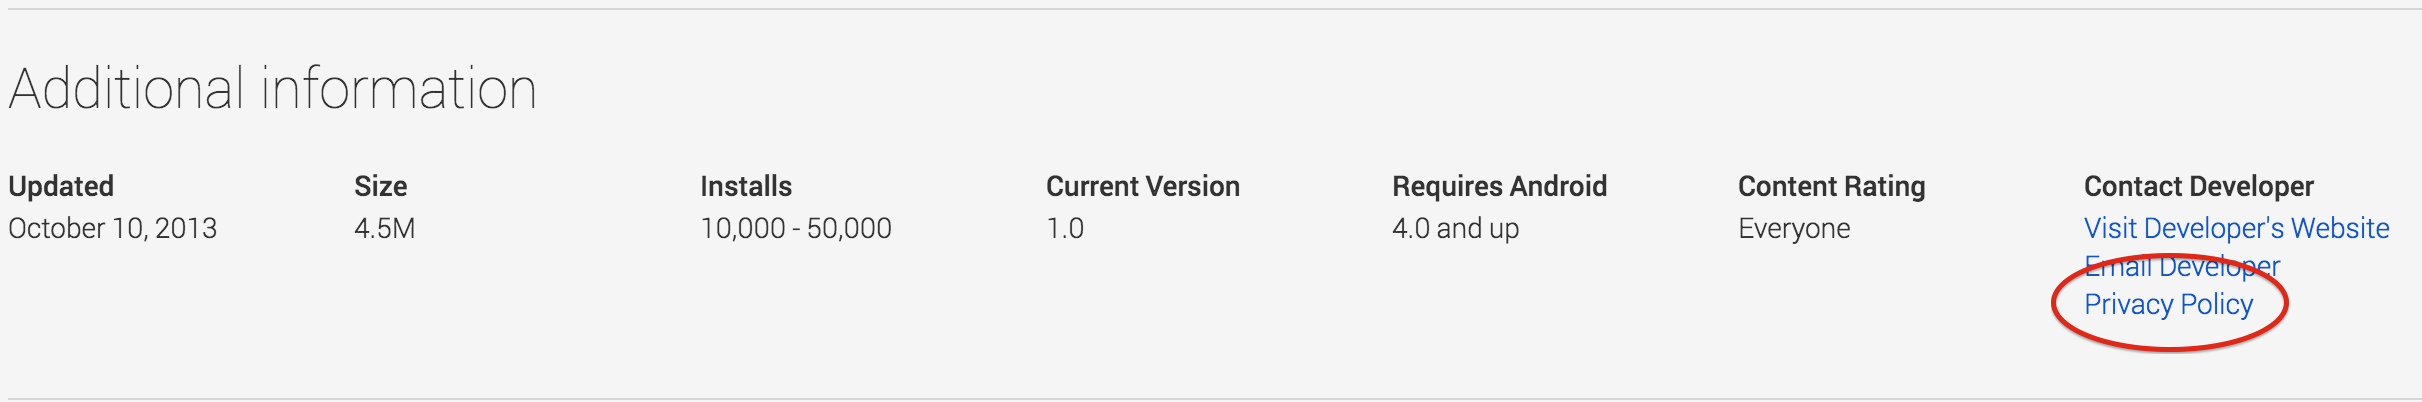
\includegraphics[width=\textwidth]{images/play-store-privacy-link}
      \caption{Privacy Policy link in the Play Store web interface}
      \label{fig:play-store-privacy-link}
\end{figure}

However, while the \texttt{AndroidManifest.xml} file is guaranteed to be present for any application on the Play Store, this does not hold true for the Privacy Policy link. 

In fact, no Play Store policies force an app to have a Privacy Policy at all.

So it can occur that either the app does not have a Privacy Policy at all, or that the developer has not inserted the Privacy Policy on the Play Store. In either case the automatic retrieval of the Privacy Policy of that app is impossible, so we will not further distinguish between them.

From the data we collected, it appears that out of the 1093 most downloaded free game apps, 39.79\% do not have a privacy policy publicly available through the Play Store.

% \todo[inline]{insert a pie chart here}

That being said, a Privacy Policy link does not guarantee the ability to retrieve an actual Privacy Policy document. The link can point to anything the developer decides, and this leads to extremely heterogeneous paths to reach the final document of our interest.

An example is redirection, which that is very common. As an example, the Privacy Policy URL for \emph{Angry Birds}, by Zynga, is:

\url{https://www.google.com/url?q=http://m.zynga.com/about/privacy-center/privacy-policy}

which redirects to

\url{http://m.zynga.com/about/privacy-center/privacy-policy}

which redirects to

\url{http://company.zynga.com/privacy/policy}

which contains the Privacy Policy document.

% \todo[inline]{Talk about the Disney example}

%%%%%%%%%%%%%%%%%%%%%%%%%%%%%%%%%%%%%%%%%%
\section{Semantic analysis}
Once the document has been retrieved, it needs to be semantically processed. For this purpose, we take advantage of Treat, a natural language processing framework for Ruby \cite{treat}. The Treat project aims to build a language-agnostic NLP framework for Ruby with support for tasks such as document retrieval, text chunking, segmentation and tokenization, natural language parsing, part-of-speech tagging, keyword extraction and named entity recognition.

The privacy policy document is firstly split into its logical subdivision using a SRX chunker, which implements the approach proposed in \cite{Milkowski:2009:USS:1987717.1987736}.

The the document is furthed split into sentences with the aid of a SRX segment, again following \cite{Milkowski:2009:USS:1987717.1987736}.


\begin{figure}[tb]
\centering
     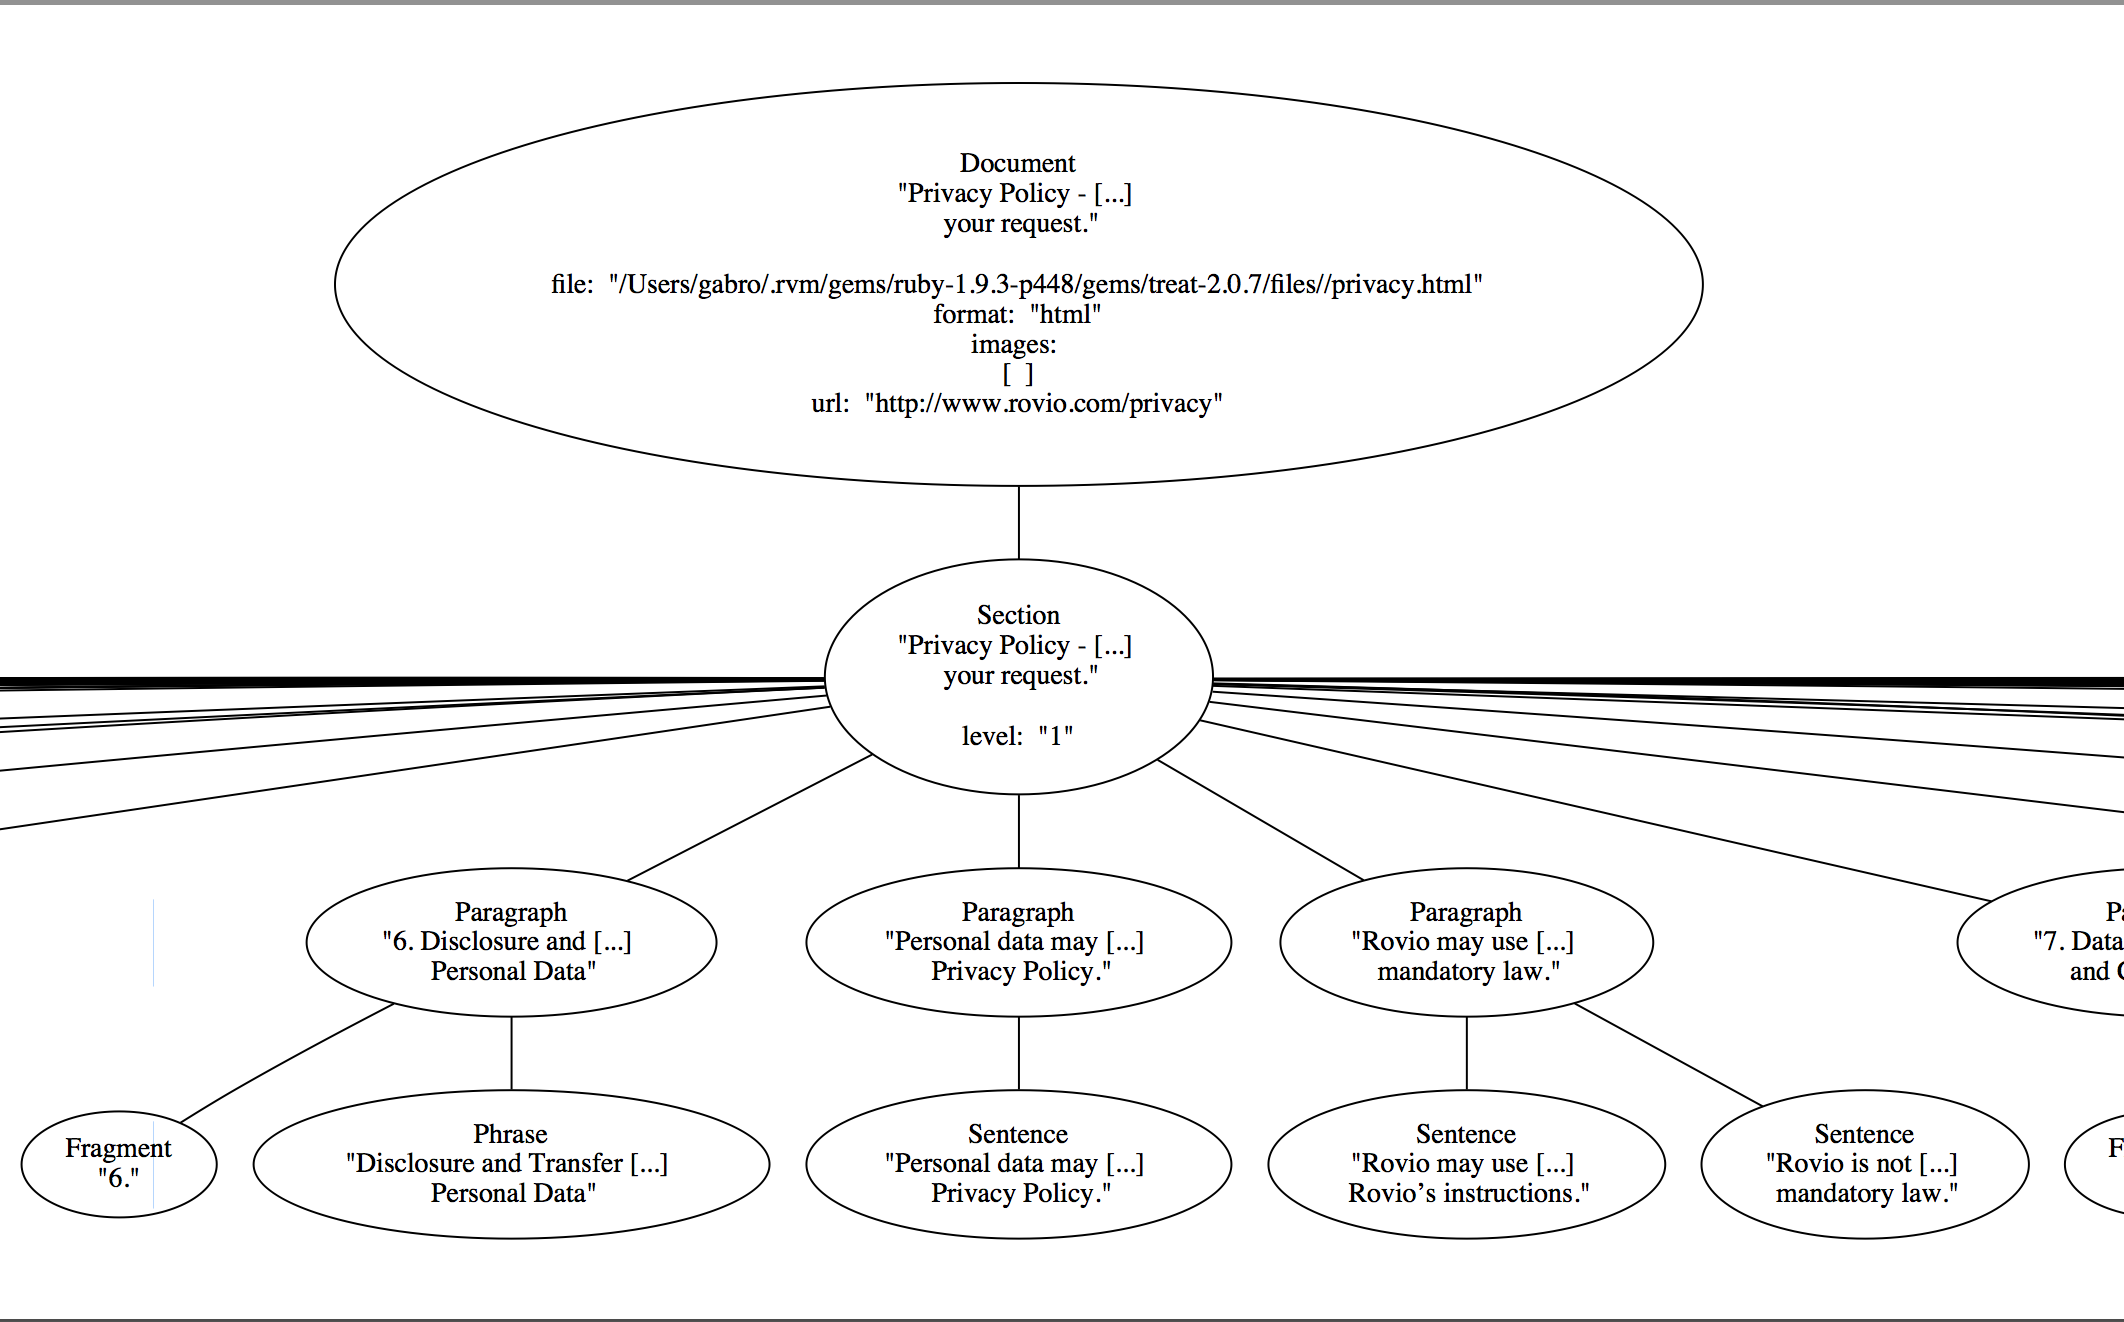
\includegraphics[width=\textwidth]{images/rovio-structure}
      \caption{Detail of Rovio's Privacy Policy structure}
      \label{fig:rovio-structure}
\end{figure}

\autoref{fig:rovio-structure} shows a detail of the semantic tree in which the original policy has been divided. Each internal node represents either paragraphs or sections of the document, whereas the leaf nodes are phrases and sentences.

Once sentences and phrases have been obtained, they can be searched for the expressions contained in the lookup table of each permission.
For example let us take the following sentence.

\begin{quote}
{\emph{``Rovio or third parties operating the ad serving technology may use demographic and \textbf{geo-location} information (for more information regarding use of Location Data see below Section 3) as well as information logged from your hardware or device to ensure that relevant advertising is presented within the Service.''}}\cite{rovio}
\end{quote}

The lookup table of \texttt{ACCESS\_COARSE\_LOCATION} contains the word ``location'', hence the above sentence will be matched and will be considered relevant to such permission.

\subsection{False positive detection}
As explained in \autoref{sec:false-positives}, we also need to search for `banned' verbal forms and exclude the sentences containing them. In order to be as general as possible, we want to consider every possible declination of the verb.
So the two main steps of this phase are:
\begin{itemize}
  \item identifying the verbs
  \item `normalizeing' each verb, in order to perform a comprehensive comparison
\end{itemize}

\subsubsection{Verb identification}
Identifying the verbs is achieved through \emph{part-of-speech tagging} (POS). POS, also called \emph{word-category disambiguation}, ``is the process of marking up a word in a text (corpus) as corresponding to a particular part of speech, based on both its definition, as well as its context—i.e. relationship with adjacent and related words in a phrase, sentence, or paragraph. A simplified form of this is commonly taught to school-age children, in the identification of words as nouns, verbs, adjectives, adverbs, etc.'' \cite{wiki:POS}. Different language taggers have been proposed over the last years: our choice fell on the most established one, i.e. the Stanford POS Tagger, which is a Java implementation of the log-linear POS tagger proposed in \cite{Toutanova:2003:FPT:1073445.1073478}.
Specifically we used the Ruby bindings provided by the aforementioned Treat framework.

As anticipated, the language tagger assigns a \emph{tag} to each word of a sentence; the tags used by the Standford Tagger are defined by the Penn Treebank tag set \cite{Marcus:1994:PTA:1075812.1075835}, in which we can find five different verb tags

\begin{itemize}
  \item VB:      Verb, base form
  \item VBD:     Verb, past tense
  \item VBG:     Verb, gerund or present participle
  \item VBN:     Verb, past participle
  \item VBP:     Verb, non-3rd person singular present
  \item VBZ:     Verb, 3rd person singular present 
\end{itemize}

Since we are interested in all the verbs of a sentence, we therefore consider all words with any of the above tags.

\subsubsection{Verbs normalization}
We are not really interested in the inflection of the verbs we are analyzing, rather we care about the concept they represent.
In order to catch all possible verbal forms, we make use of another feature of Treat: inflections. This feature allows us to perform a grammatical conjugation of an arbitrary verb.
Hence, we normalize all the verbs to their infinitive form before performing a comparison. For example, if we encounter a sentence containing the verb ``shipping'' and our ``false positive table'' includes the verb ``ship'', the sentence will be correctly excluded from the final result set.

\section{Results}
Results are discussed in detail in \autoref{sec:results}, however their collection brought up several technical challenges that required a rather sophisticated solution. The main issue is represented by the significant number of applications we want to analyze; for each one of them we need to retrieve their privacy policy, their permission list and then analyze such information.

The challenges then become:
\begin{itemize}
	\item Performing thousands of simultaneous requests to Play Store servers
	\item Performing thousands of simultaneous analysis on the same machine
\end{itemize}

The first challenge derives from Google's anti-bot protection, which results in an IP-ban in case of too many requests in a short amount of time.
The second challenges is instead an architectural limitation: spawning thousands of simultaneous computations easily hogs any personal computer's CPU, most likely leading to a system crash.

A naive approach to both challenges would be to serialize the operations, analyzing only one application at the time. However, considering an average processing time of 10 seconds per application, analyzing thousands of applications would require several hours of computation and such an architecture would not scale in case of an increased number of applications (e.g., if one would like to analyze a significant fraction of the Play Store).

What we want is then a fixed amount of computations running concurrently, in order to achieve a fast computation without hogging the computer's resources. We achieved this result taking a functional approach, namely utilizing Celluloid, a concurrent object oriented programming framework for Ruby.

Using Celluloid, we spawn a new computation for each thread - or in other terms, an \emph{actor} - which runs asynchronously and writes the results back to a MongoDB database. We use a fixed amout of actors, collectively referred to as a pool, in order to prevent the computation from using all of the computer resources, and also to prevent being banned from Google.
The result is a satisfying compromise between speed and available resources that allows to terminate the computation within reasonable time constraints.